\subsection{Random Access Memory}

\subsubsection{RAM access time}
\paragraph{Methodology}
We measured the back-to-back-load RAM access latency, because it is well accepted by most software developers and system researchers.
We use the method described in the paper \emph{lmbench: Portable Tools for Performance Analysis} to measure the memory and cache latency.
We create arrays of different sizes, we create a list of pointers to walk the list and then we walk the list like this :
\begin{verbatim}
p = *p;
\end{verbatim}

Then we created the list with different strides and did the same measurement.
For each couple of stride/array sizes we do 1,000,000 iterates through the list.
The value of the pointer p is then printed to avoid that the compiler optimize the loop and remove the instruction.

\paragraph{Predictions}
According to the \emph{Intel® 64 and IA-32 Architectures Optimization Reference Manual}
\ref{intel-archi-opti-intel64} base case latencies are :
\begin{description}
\item[L1 cache] 4 cycles
\item[L2 cache] 12 cycles
\item[L3 cache] 26-31 cycles
\end{description}
According to the ram specification the latency is about 15ns.
It's about 45 cpu cycles as the CPU is running at 3.3Ghz.


\paragraph{Results}
We are going to present the result table for stride 11 and the plotted graph for different strides from 1 to 15.

\begin{table}[h]
\begin{center}
\begin{tabular}{| r | l | l | l | r |}
\hline
Size of array 	& Hardware cost 	& Software cost 	& Prediction 	& Measured \\ \hline
512B 			&				&				&			&3.895 cycles	\\ \hline
1KB 			&				&				&			&3.886 cycles		\\ \hline
2KB 			&				&				&			&3.885 cycles		\\ \hline
4KB 			&				&				&			&3.886 cycles		\\ \hline
8KB 			&				&				&			&3.886 cycles		\\ \hline
16KB 			&				&				&			&3.888 cycles		\\ \hline
32KB 			&				&				&			&3.891 cycles		\\ \hline
64KB 			&				&				&			&5.949 cycles		\\ \hline
128KB 		&				&				&			&5.945 cycles		\\ \hline
256KB 		&				&				&			&6.209 cycles		\\ \hline
512KB 		&				&				&			&10.314 cycles		\\ \hline
1MB 			&				&				&			&10.399 cycles		\\ \hline
2MB 			&				&				&			&10.757 cycles		\\ \hline
4MB 			&				&				&			&15.585 cycles		\\ \hline
8MB 			&				&				&			&30.265 cycles		\\ \hline
16MB 			&				&				&			&37.458 cycles		\\ \hline
32MB 			&				&				&			&37.686 cycles		\\ \hline
64MB 			&				&				&			&37.092 cycles		\\ \hline
128MB 		&				&				&			&37.619 cycles		\\ \hline

\hline
\end{tabular}
\end{center}
\label{access-time-table}
\caption{RAM latency}
\end{table}
\paragraph{Success of Methodology}



\begin{figure}[h]
\begin{center}
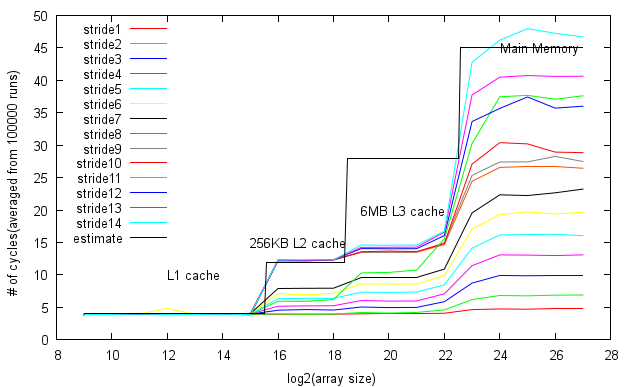
\includegraphics[scale=0.8]{memoryLatencyImage}
\end{center}
\caption {RAM latency\label{fig:access-timef}}

\end{figure}



The figure \ref{fig:access-timef} and table \ref{access-time-table} show that  //TODO actual result




\subsubsection{RAM bandwidth}
\paragraph{Methodology}
We allocated an array of 128MB so that it doesn't fit into any cache (the L3 cache is 6MB).
To make the measurement, we walked through the array by incrementing a pointer to avoid summing an index and a base pointer on each iteration.
The array is filled once before the tests to ensure that the underlying pages are really allocated and to avoid TLB misses.


For the read bandwidth an integer value was read and added to an integer stored in a register.
The resulting value is printed after the measurement to avoid a compiler optimization.
For the write bandwidth, we filled the array of an arbitrary integer value.

The optimizations are turned on to reduce the number of operations not related to the memory read.
The only other operation are an incrementation of the pointer, a comparaison and a conditional jump.
All these operations are made on values stored in registers.
The compiler options -funroll-loops also helps avoid the overhead of the loop.

The measurement unit is in cycle for 128MB and is then translated to MB/s by calculating it with the CPU clock rate.
The result is averaged on 1000 iterations.

\paragraph{Predictions}
According to the specification of the ram, the peak transfer rate is 10666 MB/s.
We are awaiting result wich should be near this value but doesn't reach this value as this is a theoritical value.
We also have a small overhead in our measurement due to the loop operations.

\paragraph{Results}
\begin{table}[h]
\begin{center}
\begin{tabular}{| l | l | l | l | l |}
\hline
Operation & Hardware cost & Software cost & Prediction & Measured \\
\hline
\end{tabular}
\end{center}

\caption{RAM bandwith\label{tab:ram-bandwith}}
\end{table}

\paragraph{Success of Methodology}




\subsubsection{Page fault service time}
\paragraph{Methodology}
In order to manually create a page fault situation, we used two really large array which are the same size as main memory.
Then we filled the first array to put it into main memory first and so that the pages are allocated.
Afterwards, we filled the second array so that the first array will be totally paged out to the swap space.
The page fault service time is going to be the time it takes to get the value of an element from the first array.

\paragraph{Predictions}


\paragraph{Results}
\begin{table}[h]
\begin{center}
\begin{tabular}{| l | l | l | l | l |}
\hline
Operation & Hardware cose & Software cost & Prediction & Measured \\
\hline
\end{tabular}
\end{center}
\caption{Page fault service time\label{tab:page-fault}}

\end{table}

As seen in table \ref{tab:page-fault} blalba
\paragraph{Success of Methodology}

